\documentclass[12pt]{article}
\usepackage[utf8]{inputenc}
\usepackage[english]{babel}
\usepackage[normalem]{ulem}
\usepackage{amsmath, amsthm, amssymb, amsfonts}
\usepackage{bm}
\usepackage{enumerate}
\usepackage[margin = 0.75in]{geometry}
\usepackage{graphicx}
\usepackage{xcolor}
\graphicspath{{doe-figures/}}

\usepackage{tikz}
\usepackage{array}
\usepackage{hyperref}
\hypersetup{
	colorlinks=true,
	linkcolor=blue,
	filecolor=magenta,      
	urlcolor=cyan,
}
\usepackage{cleveref}
\usepackage{tcolorbox}
\setlength{\parskip}{0.5\baselineskip}%
\setlength{\parindent}{1cm}%
\usepackage[stable]{footmisc}


% define new command
\newcommand{\prob}{\mathbb{P}}
\newcommand{\E}{\mathbb{E}}
\newcommand{\Var}{\text{Var}}
\newcommand{\Sample}{\mathcal{S}}
\newcommand{\R}{\mathbb{R}}
\newcommand{\C}{\mathbb{C}}
\newcommand{\N}{\mathbb{N}}
\newcommand{\Q}{\mathbb{Q}}
\newcommand{\Z}{\mathbb{Z}}
\newcommand{\transpose}{\mathsf{T}}
\newcommand{\indep}{\perp \!\!\! \perp}



\theoremstyle{definition}
\newtheorem{thm}{Theorem}
\newtheorem{lem}{Lemma}
\newtheorem{cor}{Corollary}
\newtheorem{defn}{Definition}
\newtheorem{ex}{Exercise}
\newtheorem{res}{Result}
\newtheorem{prop}{Proposition}


% define theorems and lemmas
\newenvironment{definition}{
\begin{tcolorbox}[colback=green!5!white,colframe=green!75!black, parbox = false]\begin{defn} }{\end{defn}\end{tcolorbox} }

\newenvironment{theorem}{
\begin{tcolorbox}[colback=green!5!white,colframe=green!75!black, parbox = false]\begin{thm} }{\end{thm}\end{tcolorbox} }

\newenvironment{lemma}{
\begin{tcolorbox}[colback=green!5!white,colframe=green!75!black, parbox = false]\begin{lem} }{\end{lem}\end{tcolorbox} }

\newenvironment{result}{
\begin{tcolorbox}[colback=green!5!white,colframe=green!75!black, parbox = false]\begin{res} }{\end{res}\end{tcolorbox} }

\newenvironment{proposition}{
\begin{tcolorbox}[colback=green!5!white,colframe=green!75!black, parbox = false]\begin{prop} }{\end{prop}\end{tcolorbox} }

    
\newenvironment{note}{
\begin{tcolorbox}[colback=blue!5!white,colframe=blue!75!black,title=Note, parbox = false] }{\end{tcolorbox} }

\newenvironment{remark}{
\begin{tcolorbox}[colback=blue!5!white,colframe=blue!75!black,title=Remark, parbox = false] }{\end{tcolorbox} }

\newenvironment{corollary}{
\begin{tcolorbox}[colback=blue!5!white,colframe=blue!75!black, parbox = false]\begin{cor} }{\end{cor}\end{tcolorbox} }
    
\newenvironment{example}[1][\unskip]{
\begin{tcolorbox}[colback=blue!5!white,colframe=blue!75!black, title = {Example #1}, parbox = false] }{\end{tcolorbox} }
    
\newenvironment{exercise}{
\begin{tcolorbox}[colback=red!5!white,colframe=red!75!black, parbox = false]\begin{ex} }{\end{ex}\end{tcolorbox} }




\title{\LARGE \textbf{\textcolor{purple}{Design of Experiments}}}
\author{M.Stat. $2019-2021$ Batch}
\date{\today}

\begin{document}
	
\maketitle

\begin{abstract}
    This contains some notes for the course \textit{Design of Experiments}, taught by Prof. Mausumi Bose for Master of Statistics (M.Stat.) 1st Year batch 2019-20 session. During post midsem of spring $2020$ session, the classes were suspended due to a global pandemic situation created by the breakout of Coronavirus (COVID-19). This notes are intended to cover those lost classes.
\end{abstract}
\pagebreak

\tableofcontents
\pagebreak


\section{Method of Differences}

\subsection{Introduction}\label{intro}

Let $\mathcal{A}$ be a finite additive Abelian group with $n$ elements. With every element, we associate $m$ treatments.

That is, for $a \in \mathcal{A}$, associate $a_1, a_2, \ldots, a_m$ where, $a_i$ is said to belong to the class `$i$', 
where $1 \leq i \leq m$. This implies, there are $nm$ treatments and each class has $n$ treatments.

For every ordered pair of distinct treatments, $a_i$ and $b_j$, associate the difference $a-b \in \mathcal{A}$, which is of type $(i,j)$.

\begin{definition}
	There are two types of such differences.
	\begin{enumerate}
		\item If $i = j$, such a difference is called \textbf{Pure difference}.
		\item If $i \neq j$, such a difference is called \textbf{Mixed difference}.
	\end{enumerate}		
\end{definition}


\begin{example}
Let us consider, $\mathcal{A} = \{0,1,2,3,4,5,6\}$

Suppose $m = 1$, Consider the triplet $(0,1,3)$. Look at all pairwise differences; $\{6,4,1,2,5,3\}$, \textit{i.e}, all differences occur once. Hence, this $(0,1,3)$ becomes a block. 

\begin{note}
	For $m = 1$, it is easy. But, for $m > 1$, things become complex.
\end{note}

\end{example}

\subsection{Method of differences for constructing BIB designs}

The notions of ``pure difference'', ``mixed difference'', symmetrically repeated differences and how to obtain such differences arising from a given set of treatments have been discussed (\hyperref[intro]{above}). We continue from there.\par

\begin{note}
	A finite additive Abelian group $\mathcal{A}$ has $n$ elements: $a^{(0)}, a^{(1)}, \ldots, a^{(n-1)}$ and each $a^{(w)}$ there corresponds to $m$ treatments of the form $a^{(w)}_{i}, 0 \leq w \leq n-1, 1 \leq i \leq m$. Thus, there are $v = mn$ treatments with $m$ classes, each class having $n$ treatments.
\end{note}

\subsubsection{Notion of ``developing a block''}

Let $B_j$ be a block of $k$ \textbf{distinct} treatments. From $B_j$, construct a new block $B_{j, \theta}$ by replacing each treatment $a^{(w)}_{i}$ in $B_j$ by the treatment $a_i^{(u)}$, where $$ a^{(u)} = a^{(w)} + \theta, \theta \in \mathcal{A}. $$ 
Thus, we can get a set of $n$ blocks from $B_j$. These blocks are said to be \textit{obtained by developing $B_j$}. Trivially, $B_{j, 0} = B_j$.

\begin{example}
	Let $\mathcal{A} =$ residue class mod $7$ i.e, $\mathcal{A} = \{0,1,2,3,4,5,6\}$. Let $m = 1$; clearly, $v = 7$. Consider the block $B_1 = \{0, 1, 3\}$. Then, 
\begin{align*}
	B_{1,0} &= B_1 \\  
	B_{1,1} &= \{1,2,4\}  &B_{1,2} &= \{2,3,5\} &B_{1,3} &= \{3,4,6\} \\
	B_{1,4} &= \{4,5,0\} &B_{1,5} &= \{5,6,1\} &B_{1,6} &= \{6,0,2\}
\end{align*}
These $7$ blocks are obtained by ``developing'' $B_1$. 
\end{example}

Now we consider the main theorem regarding such construction of these blocks.

\begin{theorem}\label{thm:difference-1}
	Suppose $p$ blocks $B_1, B_2, \ldots, B_p$ can be formed with the $v$ treatments $a^{(w)}_{i}, 0 \leq w \leq n-1, 1 \leq i \leq m$; such that, 
		\begin{enumerate}
			\item[(i)] each $B_j$ has $k$ distinct treatments, $1 \leq j \leq p$. 
			\item[(ii)] exactly $r$ of the treatments in $B_1, B_2, \ldots, B_p$ belong to each of the $m$ classes.
			\item[(iii)] the differences arising from $B_1, B_2, \ldots, B_p$ are symmetrically repeated, i.e, each possible difference is repeated a constant number of times, say $\lambda$. \par 
			Then the blocks obtained by developing $B_1, B_2, \ldots, B_p$ forms the block of a BIB design with $v = mn, b = np, r, k, \lambda$.
		\end{enumerate}
\end{theorem}

Note that, to identify the differences arising from $B_1, B_2, \ldots, B_p$ which are symmetrically repeated, the pairwise differences are obtained between treatments within each block, but we do not consider the differences between treatments in two  different blocks. Once, all these pairwise differences obtained from all the blocks are considered together, then each difference should appear exactly once. The blocks $B_1, B_2, \dots B_p$ are called the initial blocks, which on development give all blocks of the BIB design.

Consider the following example to make things clearer.

\begin{example}
    Consider the abelian group of residue classes mod $5$ as $\left\{0,1,2,3,4,5\right\}$ and let $m=3$. Then $n=5$ and $m=3$ together gives the $v=15$ treatments denoted as 
    $$0_1, 0_2, 0_3,  \quad 1_1, 1_2, 1_3, \quad 2_1, 2_2, 2_3,  \quad 3_1, 3_2, 3_3, \quad 4_1, 4_2, 4_3$$
    
    Now, consider the following initial $p = 7$ blocks.
    
    \begin{enumerate}
        \item $B_1 = (1_1, 4_1, 0_2)$
        \item $B_2 =  (2_1, 3_1, 0_2)$
        \item $B_3 = (1_2, 4_2, 0_3)$
        \item $B_4 = (2_2, 3_2, 0_3)$
        \item $B_5 = (1_3, 4_3, 0_1)$
        \item $B_6 = (2_3, 3_3, 0_1)$
        \item $B_7 = (0_1, 0_2, 0_3)$
    \end{enumerate}
    
    Note that, these blocks satisfy the conditions of the theorem.
    \begin{enumerate}
        \item[(i)] Each block has $3$ treatments, so $k = 3$.
        \item[(ii)] There are $7$ treatments in each of the $3$ classes over all the $7$ blocks, i.e., $r=7$.
        \item[(iii)] If you obtain the pairwise differences from each of these blocks, and consider them all, you will find the differences symmetrically repeated.
        Note that here are in all 9 types of differences:
        \begin{enumerate}
            \item[(a)]  $3$ pure differences:  $[1,1], [2,2], [3,3]$
            \item[(b)] $6$ mixed differences: $[1,2], [1,3], [2,3], [2,1], [3,1], [3,2]$
        \end{enumerate}
        where each pure difference can be $1, 2, 3$ or $4$, while each mixed difference can be $0, 1, 2, 3, 4$. Now, from $B_1$ the differences are $3$ and $2$ of type $[1,1]$ ,  $1$ and $4$ of type $[1,2]$,  $4$ and $1$ of type $[2,1]$. From $B_2$ the differences are $1$ and $4$ of type $[1,1]$, $2$ and $3$ of type $[1,2]$ and $3$ and $2$ of type $[2,1]$, etc. If you get the differences from all $7$ blocks you will see that all the differences (of each type) come exactly once each, the last $B_7$ contributing the difference 0 to each one of the mixed differences.
    \end{enumerate}
    So these 7 initial blocks can be developed to give a BIB design with $v= mn = 15$, $b= np = 35$, $r=7$, $k=3$, $\lambda = 1$.
\end{example}

Now, let us work out some more examples, which are left as exercises.

\begin{exercise}
	Check that the block $B_1$ satisfies the conditions of the theorem for $m = 1$, $n = 7$. So the $7$ blocks developed in the example before, gives a BIBD with $v = 7, b = 7, k = 3, r = 3, \lambda = 1$.
\end{exercise}

\begin{exercise}
	With $\mathcal{A} \equiv \text{residue class modulo $13$}$; and $m = 1$; check that the block $B_1 = (0, 1, 3, 9)$ will give a BIBD. Find its parameters.
\end{exercise}

\begin{example}
	Suppose $\bm{v = 6u+1}$ is a prime/prime power. Let, $\text{GF}(v)$ be the Galois Field of order $v$ and $x$ be a primitive element of $\text{GF}(v)$. Then check that the blocks $B_0, B_1, \ldots, B_{m-1}$ given by: 
	$$ B_j = (x^j, x^{2u+j}, x^{4u+j}), 0 \leq j \leq u-1 $$ satisfy conditions of \hyperref[thm:difference-1]{Theorem 1} and lead to a BIB design with $v=6u+1$, $b=u(6u+1)$, $r=3u$, $k=3$, $\lambda=1$.
	
	\begin{exercise}
	    Try this with $m = 3$ and use $2$ as a primitive element of $\text{GF}(19)$. Also try with $m = 2$.
	    \label{ex-3}
	\end{exercise}
\end{example}

\begin{proof}
	\textit{The proof of Theorem \ref{thm:difference-1} is skipped for now, and will be discussed in class if time permits}
\end{proof}

Please consider the following notes.

\begin{note}
	\begin{itemize}
		\item Please work out all the exercises in full to understand the method properly.
		\item Note that in Exercise \ref{ex-3}, if you take $m = 1$, then you get the blocks of what is given in the example before. 
		\item  The method in Exercise \ref{ex-3} always give BIBD with $k = 3$ and $\lambda = 1$. These are members of \textbf{Steiner's Triple Systems}, where every pair of objects appear in exactly one triplet/block.
	\end{itemize}
\end{note}

\begin{exercise}
	\textbf{This is a thinking exercise mostly}
	Are designs given by method described in Exercise \ref{ex-3} resolvable BIB designs? (\textit{Recall:} a BIB design is resolvable if its blocks can be partitoned into $\tau$ sets of blocks, each set having $\dfrac{b}{\tau}$ blocks, such that every set contains every treatment exactly once.)
\end{exercise}

\newpage 

\section{Introduction to Factorial Designs}

The first part of this section is taken from the book \textit{Design and Analysis of Experiment} by Douglas C. Montgomery (\href{https://drive.google.com/open?id=1ZmF_RCztbGjLKawqP9l1Yo7ZsrOoI9ev}{Link})

Many experiments involve the study of the effects of two or more factors. In general, factorial designs are most efficient for this type of experiment. By a factorial design, we mean that in each complete trial or replicate of the experiment all possible combinations of the levels of the factors are investigated. \textit{For example}, if there are $a$ levels of factor $A$ and $b$ levels of factor $B$, each replicate contains all $ab$ treatment combinations. When factors are arranged in a factorial design, they are often said to be \textbf{crossed}. 

\begin{note}
\textbf{Ref. ma'am:} I prefer the nomenclature \textit{Factorial Experiments} instead of Factorial Designs since factorial experiments are a way of doing experiments where there are several factors of interest, each factor having a number of levels,  and each experimental unit receives a combination  of these factors at different levels. (This can be contrasted to  varietal experiments where there is only one treatment factor of interest, at different levels, say $v$ levels. For example, in block designs there is the treatment factor of interest, (we say there are $v$ treatments) and the block effect is the nuisance parameter. ) \par

If a factorial experiment has m factors $F_1, F_2, ...F_m$ at $s_1, s_2, ..., s_m$ levels, then each experimental unit receives a treatment combination of the form $(i_1,i_2, \ldots ,i_m)$, where  $i_j = 1, 2, ...,s_j$; and $j=1, 2, ..., m$. So now there are in all the product $s_1s_2..s_m$ ($=v$, say) treatment combinations. These $v$ combinations can be used in different designs as per the experimental material available, \textit{e.g}., if $v$ homogeneous units are available, we can run the factorial experiment  as a CRD,  else as  RBD, LSD, or BIBD , or any other design. 

\end{note}


There are two types of effect in a Factorial Experiment. Figure \ref{fig:interaction-factorial} illustrates the idea.

\begin{figure}[h]
    \centering
    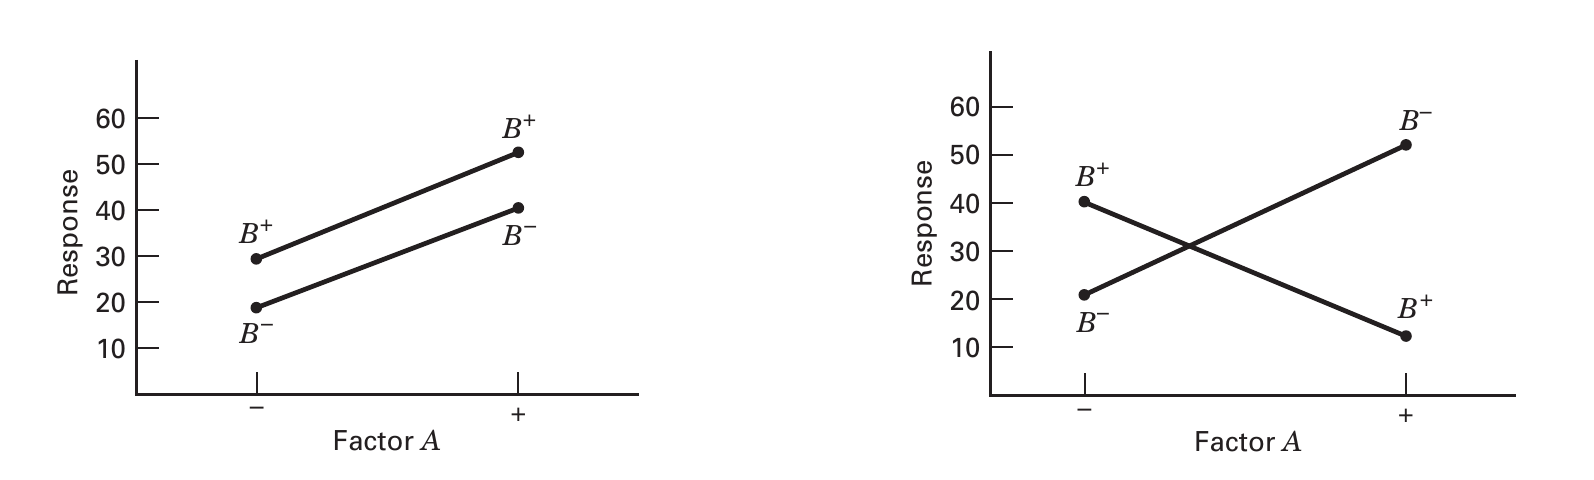
\includegraphics[width = \textwidth]{interaction-factorial.png}
    \caption{[Left] A factorial experiment without interaction; [Right] A factorial experiment with interaction}
    \label{fig:interaction-factorial}
\end{figure}

\begin{enumerate}
    \item \textbf{Main Effect:} The main effect of a treatment factor $A$ is basically the average change in response when an experimental units is assigned from a low level of $A$ to a higher level of $A$, where the averaging it done over all levels of the other factor.
    \item \textbf{Interaction Effect:} The interaction effect of a treatment factor combination (unordered set) $\left\{A, B\right\}$ is basically the change of (change in response from a factor going from low level to a higher level), at different levels of the other factor(s). 
\end{enumerate}


\subsection{Advantage of Factorial Design}

The advantage of factorial designs can be easily illustrated. Suppose we have two factors $A$ and $B$, each at two levels. We denote the levels of the factors by $A_{+}$, $A_{-}$, $B_{+}$, and $B_{-}$. Information on both factors could be obtained by varying the factors one at a time. The effect of changing factor $A$ is given by $A_{+}B_{+} - A_{-}B_{+}$, and the effect of changing factor $B$ is given by $A_{-}B_{+} - A_{-}B_{-}$. Because experimental error is present, it is
desirable to take two observations, say, at each treatment combination and estimate the effects of the factors using average responses. Thus, a total of six observations are required, if we perform this in the one at a time manner.

Compared to that, if a factorial experiment is conducted, we would have $4$ treatment factor combination, $A_{+}B_{+}, A_{+}B_{-}, A_{-}B_{+}$ and $A_{-}B_{-}$. Note that, then we also had two differences to estimates the main effect of factor $A$, namely, $A_{+}B_{+} - A_{-}B_{+}$ and $A_{+}B_{-} - A_{-}B_{-}$. Hence, we would be able to estimate these effects with atleast as the same precision as before. However, in total, we are only in need of $4$ observations.

In this manner, for more than two factors, or factors with more than two levels, we can save up a lot, by resorting to Factorial Experiments.


\subsection{Two Factor Factorial Experiment}

Here, we shall be considering a two factor factorial experiment, with a completely randomized design assigned to the experiment. This basically means, the experimental units are assigned to the treatment combinations randomly, and each combination is repeated same number of times.

A mathematical model for this is as follows:
$$
y_{ijk} = \mu + \tau_i + \beta_j + (\tau\beta)_{ij} + \epsilon_{ijk}
\begin{cases}
i & = 1, 2, \dots a\\
j & = 1, 2, \dots b\\
k & = 1, 2, \dots r
\end{cases}
$$

This model description is very similar to a Randomized Block Design with repeated observations, however, the key thing to notice here is that both $\tau_i$ and $\beta_j$ are variables of interest here, not just  nuisance parameters due to blocking factor.

Let us introduce some notations as follows:
  $$G = \bar{y}_{\cdot\cdot\cdot} = \frac{\sum_{i,j,k} y_{ijk}}{abr}  \quad
  T_i = \bar{y}_{i\cdot\cdot} = \frac{\sum_{j,k} y_{ijk}}{br} \quad
  B_j = \bar{y}_{\cdot j \cdot} = \frac{\sum_{i,k} y_{ijk}}{ar} \quad (TB)_{ij} = \bar{y}_{ij\cdot} = \frac{\sum_{k} y_{ijk}}{r}$$
    
\begin{align*}
    SS_T & = \sum_{i,j,k} \left( y_{ijk} - G \right)^2  = \sum_{i,j,k} y_{ijk}^2 - abr G^2\\
    SS_A & = br \sum_{i} (T_i - G)^2 = br \sum_{i}T_i^2 - abr G^2\\
    SS_B & = ar \sum_{j} (B_j - G)^2 = ar \sum_{j}B_j^2 - abr G^2\\
    SS_{AB} & = r \sum_{i, j} \left( TB_{ij} - T_i - B_j + G \right)^2 = r\sum_{i, j} TB_{ij}^2 - br \sum_{i} T_i^2 - ar \sum_{j} B_j^2 + abr G^2 \\
    SS_{E} & = \sum_{i, j, k} \left( y_{ijk} - TB_{ij} \right)^2
\end{align*}

Then, we have the estimates;
$$
\hat{\mu} = G  \qquad
\hat{\tau}_i = T_i  \qquad 
\hat{\beta}_j = B_j  \qquad
\hat{\tau\beta}_{ij} = (TB)_{ij}
$$

and the ANOVA table is given in Table \ref{tbl:anova-two-factor}.

{\renewcommand{\arraystretch}{2.75}% for the vertical padding
\begin{table}[h]
    \centering
    \begin{tabular}{|>{\centering\arraybackslash}m{3.5cm}|c|c|c|}
        \hline
         \textbf{Source of Variation} & \textbf{Sum of Squares} & \textbf{Degrees of Freedom} & \textbf{Expected Mean Square}\\
         \hline
         Main effect of $A$ & $SS_A$ & $(a-1)$ & $\sigma^2 + \dfrac{bn \sum_i \tau_i^2}{(a-1)}$\\
         Main effect of $B$ & $SS_B$ & $(b-1)$ & $\sigma^2 + \dfrac{an \sum_j \beta_j^2}{(b-1)}$\\
         Interaction effect between $A$ and $B$ & $SS_{AB}$ & $(a-1)(b-1)$ & $\sigma^2 + \dfrac{n \sum_{i,j} (\tau\beta)_{ij}^2}{(a-1)(b-1)}$\\
         Error & $SS_{E}$ & $ab(n-1)$ & $\sigma^2$\\
         \hline
        \textbf{Total} & $SS_{T}$ & $abn - 1$ & \\         
         \hline
    \end{tabular}
    \caption{ANOVA Table}
    \label{tbl:anova-two-factor}
\end{table}
}


% notes day 3 from here

\subsection{Inference for General Factorial Experiments}

\begin{definition}
    A factorial experiment involving $n (\geq 2)$ factors $F_1,\ldots,F_n$ at levels  $s_1,\dots, s_n$ respectively. Such an experiment is called  an $s_1 \times \cdots \times s_n$ factorial experiment, or an $s_1 \times \cdots \times s_n$ factorial.
    If $s_1= \cdots = s_n = s$, it is called a symmetrical  factorial, denoted by $s^n$ factorial, otherwise it is called an asymmetrical factorial.
\end{definition}

For example a $2\times 3\times 2$ factorial has 3 factors at levels $2,3,2$, respectively. If we have 3 factors $A, B$ and $C$, each having $2$ levels, then we would have a symmetric $2^3$ factorial.

For $1 \leq i \leq n$, the $s_i$ levels of the  factor $F_i$ are denoted by $s_i$ symbols, say  $0, 1, \ldots, s_i-1$.

When a factorial experiment is run as any design, as seen in earlier notes, a treatment combination (i.e., a combination of the levels of the n factors) is applied to each unit.  A typical treatment combination is represented by an ordered n-tuple $ j_1 , \ldots, j_n$, where  $j_i \in \{0, \ldots, s_i-1\}, \leq i \leq n$.  Thus, altogether there are $\prod_{i=1}^n s_i\left(=v\right.$ , say) treatment combinations in all. So there will be a total of $v-1$ degrees of freedom for treatments.

For example, for a $2\times 3$ factorial, there are 6 treatment combinations given by the ordered pairs: $$00, 01, 02, 10, 11, 12$$ 

For a $3\times 2\times 2$ factorial, the 12 treatment combinations are denoted as the ordered triplets; $$000, 001, 010, 011,  100, 101, 110, 111, 200, 201, 210, 211$$ 

Let  $\tau (j_1, \ldots,  j_n)$  denote  the  treatment  effect  corresponding  to  a  treatment combination $j_1, \ldots, j_n$. These treatment effects are unknown parameters in the context of a factorial experiment.  

In the context of varietal experiments, we had $\tau_1, \ldots, \tau_v$ as the treatment parameters. A treatment contrast was defined in terms of these $\tau_i$'s. Similarly, we can define contrasts in the context of factorial experiments also.

\begin{definition}
    A linear parametric function
    \begin{equation}
        L = \sum_{j_1=0}^{s_{1-1}} \cdots \sum_{j_n=0}^{s{_{n-1}}} l(j_1, \ldots j_n) \tau(j_1, \ldots j_n)
    \end{equation}
    where $l(j_1, \ldots j_n)$ are real numbers not all zero, such that 
    \begin{equation}
        \sum_{j_1=0}^{s_{1-1}} \cdots \sum_{j_n=0}^{s{_{n-1}}}  l(j_1, \ldots j_n) =0
    \end{equation}
    is called a \textbf{treatment contrast}. 
\end{definition}

However, in factorial experiments, this general treatment contrast is not of much interest, we are interested in the treatment contrasts belonging to specific factorial effects like the main effects and interaction effects.  

\begin{definition}
    A treatment contrast
    $$L = \sum_{j_1=0}^{s_1-1} \cdots \sum_{j_n=0}^{s_n-1} l(j_1, \ldots j_n) \tau(j_1, \ldots j_n) $$
    is said to belong to the factorial effect $F_{i_1}\ldots F_{i_g}$, for $(1 \leq i_1 < \dots < i_g \leq n; 1\leq g \leq n)$ if
    
    \begin{enumerate}
        \item[(i)] $l(j_1 . . . j_n)$ depends only on $j_{i_1}, \ldots, j_{i_g}$.
        \item[(ii)] Writing $l(j_1 . . . j_n) = \bar{l}(j_{i_1}, \ldots, j_{i_g} )$ in view of (i) above, the sum of $\bar{l}(j_{i_1}, \ldots, j_{i_g} )$ separately over each of the arguments $j_{i_1}, \ldots, j_{i_g} $ is zero.
    \end{enumerate}
    \label{defn:contrast-factorial-effect}
\end{definition}


A factorial effect  $F_{i_1} \ldots F_{i_g} $ as defined above, will be called a \textbf{Main Effect} if it involves only one factor, i.e., $ g=1$; and will be called an \textbf{Interaction effect} if it involves more than one factor, i.e., $g > 1$. For example, $F_5, F_3$ are main effects, while $F_1F_2,  F_3F_5F_6$  are interaction effects of 2 and 3 factors respectively.  

Thus there are $n$ main effects and $\displaystyle \binom{n}{g}$ many $g-$factor interactions. So the total number of factorial effects is $\displaystyle \sum_{x=1}^n \binom{n}{x}  = 2^n-1$.

\begin{example}
    This example based on $2^2$ factorial is to illustrate the contrasts belonging to different effects under the general notion introduced.
    We have the 4 treatment combinations, $00, 01, 10, 11$.
    
    \begin{enumerate}
        \item[(a)]     To find a contrast belonging to main effect $F_1$, we have to take $g=1$ and $i_1=1$ in  $L$ in  Definition \ref{defn:contrast-factorial-effect} to get 
    $$\sum_{j_1=0}^{s_1-1} \cdots \sum_{j_n=0}^{s_n-1} \bar{l}(j_1) \tau(j_1, \ldots j_n) $$
    where $\sum_{j_1=0}^{s_1-1} \bar{l} (j_1) =0$. Here $\bar{l}(j_1)$ is written to reflect the fact that the values depend only on levels of $F_1$ by (i). We need to choose the $\bar{l}(j_1)$ values  satisfying (i) and (ii) of Definition \ref{defn:contrast-factorial-effect}.
    Suppose we take $\bar{l}(1)=1$ and $\bar{l}(0)=(-1)$.  Check that with this choice, (i) and (ii) are satisfied. So,
    $$L(F_1) = [\tau(10) - \tau(00) + \tau(11)-\tau(01)]$$ is a contrast belonging to main effect $F_1$.
    \end{enumerate}
\end{example}

\begin{example}[(Continued)]
    From earlier notes recall that the contrast belonging to main effect  $F_1$ is obtained by taking the average of the effects of changing$ F_1$ from 0 to 1, while keeping $F_2$ fixed at 0 and 1, respectively. i.e., in this notation, the  main effect of $F_1$ is 
    $$ = \frac{1}{2}[\{\tau(10)-\tau(00)\} + \{\tau(11)-\tau(01)\}]$$ See that this matches (apart from the divisor 2) what we get as $L_1$ from the above following Definition \ref{defn:contrast-factorial-effect}.
    
    \begin{enumerate}
    \item[(b)] Check that the contrast belonging to main effect $F_2$ is given by
    $$L(F_2) = [\tau(01) - \tau(00) + \tau(11)-\tau(10)].$$
    Also check that it matches our earlier definition of main effect contrast belonging to $F_2$, (apart from divisor 2).
    
    \item[(c)] To find the contrast belonging to interaction $F_1F_2$, take $g=2, i_1=1, i_2=2$ in Definition 1. Thus a treatment contrast belonging to $F_1F_2$ will be of the form  
    $$\sum_{j_1=0}^{s_1-1} \cdots \sum_{j_n=0}^{s_n-1}  \bar {l}(j_1 j_2) \tau(j_1, \ldots j_n), $$ 
    where the $\bar{l}(j_1j_2)$ values must depend on both $F_1$ and $F_2$ and 
    $$ \sum_{j_1=0}^{s_1-1} \bar{l}(j_1j_2) =0, {\mbox{ for each }}   j_2, \  0\leq j_2 \leq s_2-1,$$ 
    and
    $$ \sum_{j_2=0}^{s_2-1} \bar{l}(j_1j_2) =0, {\mbox{ for each }}  j_1, \ 0\leq j_1 \leq s_1-1.$$	
    Take $\bar{l}(00)=\bar{l}(11)=1, \bar{l}(01)=\bar{l}(10)=-1.$ 
	Check that this choice satisfies (i) and (ii) and so  a contrast belonging to $F_1F_2$  is 
    $$L(F_1F_2) = [\tau(11) - \tau(01) - \tau(10)+ \tau(00)]$$
    Again, by means of previous section, the interaction $F_1F_2$ was explained  as the influence of the level where $F_2$ is held fixed on the effect of a level change of $F_1$.Thus it was measured by the difference between the effect of changing levels of $F_1$ when  $F_2$ is held at level 1 and the effect of changing levels of $F_1$ when $F_2$ is held at level 0. i.e., equal to $$ = \frac{1}{2}[\{\tau(11)-\tau(01)\} - \{\tau(10)-\tau(00)\}]$$ Note that what you get as $ L(F_1F_2)$ above is same as this. (apart from divisor 2).
    \end{enumerate}
\end{example}

\begin{example}[(Continued)]
    Also note that the interaction $F_1F_2$ could as well be thought of as the influence of the level where $F_1$ is held fixed on the effect of a level change of $F_2$. This is seen from  the fact that the expression above remains invariant when the roles of the two factors are interchanged.
\end{example}

The following exercise should help you work out an example yourself.

\begin{exercise}
    Write down $L(F_1), L(F_2), L(F_1F_2) $ for a $2\times 3$ factorial. Check that you can get two sets of solutions of $\bar{l}(j_1j_2) $  for $F_2$ and also for $F_1F_2$, showing that there are two contrasts for main effects $F_2$ and also 2 contrasts for interaction  $F_1F_2$.     
\end{exercise}
 
\begin{remark}
    \begin{enumerate}
        \item The multiplier $\frac{1}{2}$ used in earlier notes and in many other texts on DOE,  will be ignored from now on. This is because in statistical applications, we can always scale the contrasts suitably. In fact, if this multiplier  $\frac{1}{2}$ is replaced by any other (non-zero) constant, we would still get contrasts proportional to our expressions for $L(F_1), L(F_2)$ or  $L(F_1F_2)$.
        \item This form of contrasts is common in most text books. However, if we have to obtain the coefficients for a factorial which has a large number of factors at different numbers of levels, this process is cumbersome.  So an alternative is welcome.
    \end{enumerate}
\end{remark}

\subsubsection{Introduction to Kronecker Calculus for Factorials}

In this part, a new way of studying factorials using Knocker calculus is introduced.\footnote{In fact, the part on factorials till now is a revision of basic factorials from the course on Design of Experiments you had in B. Stat. Year III.}

\begin{note}
     The material in the notes on preliminaries on factorials using the Kronecker Calculus is based  (in a simplied form) on Chapters 2 and 3 of the book: \textit{A Calculus for factorial arrangements, by Gupta and Mukerjee, Springer Lecture Notes in Statistics, New York. (1989)}
\end{note}


Suppose all the $v$ treatment combinations are ordered lexicographically. e.g.,   for a $4\times 5$ factorial  they are written in the order 
$$00, 01, \ldots, 04, 10, 11, \ldots , 14, \ldots , 30, 31, \ldots, 34$$ 
Let $\tau$  be a $v\times 1$ vector of the treatment effects $\tau(j_1 \dots j_n) \quad  (0 \leq j_i \leq  s_i-1, \quad  1 \leq  i \leq n)$ written in lexicographic order. For example, for a $4\times 5$ factorial, the vector of treatment effects is $$\tau = \left(\tau(00), \tau(01), \ldots, \tau(04), \tau(10), \tau(11), \ldots , \tau(14), \ldots , \tau(30), \tau(31), \ldots, \tau(34)\right)^{\transpose}$$

It should be an obvious fact that, any treatment contrast can then be expressed as $l^{\transpose}\tau$ , where $l$ is a nonnull $v \times 1$ vector whose elements add up to zero. Recall that the total  number of factorial effects  is $2^n-1$. Now, consider the set  $\Omega$ of all non-null binary $n$-tuples. Clearly, $\Omega$  has cardinality $2^n-1$. So, we can establish a one-to-one correspondence between the set of all
factorial effects and the set $\Omega$ and express the factorial effect $F_{i_1} \ldots F_{i_g} $ as $F(x)$, where $x = x_1 x_2\ldots x_n$ and  $x_i=1$ if $i \in \{i_1, i_2, \ldots i_g\}$ and is zero otherwise. 

Let us consider two examples to make it more clear.

\begin{example}
    \begin{enumerate}
        \item For $n=2$, main effects $F_1, F_2$ and interaction effect $F_1F_2$  can be represented as $F(10), F(01)$ and $F(11)$, respectively.
        \item For $n=3$, main effect $F_3$ becomes $F(001)$, interaction $F_2F_3$ becomes $F(011)$.
    \end{enumerate}
\end{example}

Now, we will see how to  obtain factorial contrasts satisfying Definition \ref{defn:contrast-factorial-effect} in an easy way by  using the Kronecker product of the $P$ matrices studied earlier. These $P$ matrices are basically the coefficients corresponding to the orthonormal Helmert Contrasts. Recall the $(v-1)\times v$ matrix $P$ studied earlier in the context of varietal designs with $v$ treatments. This $P$  is such that the matrix 
$$\begin{pmatrix}
\dfrac{\mathbf{1}_v^{\transpose}}{\sqrt{v}}\\
P
\end{pmatrix}$$ 
is an orthogonal matrix, leading to $P\mathbf{1}_v=0$ and rank$(P) =(v-1)$. In the same way, in the context of factorials, consider the  $(s_i-1)\times s_i$ matrix, denoted by $P_i$, say,  which is such that the matrix 
$$\begin{pmatrix}
\dfrac{\mathbf{1}_{s_i}^{\transpose}}{\sqrt{s_i}}\\
P_i
\end{pmatrix}$$ 
is an orthogonal matrix, leading to $P_i \mathbf{1}_{s_i}=0$ and rank($P_i$)$=(s_i - 1)$ for all $i = 1, 2, \dots n$.


Now, for any $x=x_1, \ldots x_n \in \Omega$, define 

$$P^x =P_1^{x_1} \otimes P_2^{x_2} \otimes \ldots \otimes P_n^{x_n},$$
where, for $1\leq i \leq n$,

$$
P_i^{x_i} = \begin{cases}
\mathbf{1}_{s_i}^{\transpose} & \text{ if } x_i = 0\\
P_i & \text{ if } x_i = 1
\end{cases}
$$

and $\otimes$ denotes Kronecker product. Clearly, $P^x$ is a matrix with $s(x)$ rows and $v(=\prod_{i=1}^n s_i$) columns, where 
$$ s(x) = \prod_{i=1}^n (s_i-1)^{x_i}.$$
 
Again, recall that in the context of varietal designs,  the rows of $P\tau$ represented a full set of orthonormal treatment contrasts. In the context of factorials we have the following result

\begin{theorem}
    For all $x \in \Omega$, the rows of $P^x\tau$ represent a full set of orthonormal contrasts belonging to the factorial effect $F(x)$.
    \label{thm:result1-note3}
\end{theorem}
 
\begin{proof}
    Proof is left as an exercise with following hints:
    \begin{enumerate}
        \item[(a)] Show that $P^x \mathbf{1}_v = 0$. 
        Remember that $\mathbf{1}_v = \mathbf{1}_{s_1}\otimes  \mathbf{1}_{s_2} \otimes \ldots \otimes  \mathbf{1}_{s_n}$
        This shows the rows of $P^x\tau$ are contrasts.
        \item[(b)] Show that condition (i) of Definition \ref{defn:contrast-factorial-effect} is satisfied by definition of $P^x$. This shows it belongs to $F(x)$.
        \item[(c)] Show that rank$(P^x) = (v-1)$ (Remember rank$(A\otimes B )$ = rank $(A)\times$ rank$(B)$). This shows full set.
    \end{enumerate}
\end{proof}

\begin{example}
    For a $3\times 4\times 2$ factorial, the contrasts belonging to main effect $F_1$ (or effect $F(100)$) is given the rows of  $P^{100} \tau = (P_1\otimes \mathbf{1}^{\transpose}_{s_2} \otimes \mathbf{1}^{\transpose}_{s_3})\tau, $ where $\mathbf{1}_{s_2}= \mathbf{1}_4$ and  $\mathbf{1}_{s_3}= \mathbf{1}_2$.  So it is easy to write down the contrasts, knowing the form of the matrix $P_1$. Note that  $P^{100} \tau$ has 2 rows and 12 columns and its rows give the two independent contrasts belong to main effect $F_1.$ Similarly, contrasts belong to interaction $F_2F_3$ (i.e.,  effect $F(011)$) are given by  $P^{011} \tau$.
    \label{example:factorial-1}
\end{example}

\begin{exercise}
    Write down the contrasts of the previous example using this Kronecker approach.
\end{exercise}

\begin{exercise}
    Show that any two treatment contrasts belonging to  different factorial effects are orthogonal.
    \label{exe:factorial-orthogonal}
\end{exercise}


To complete the previous exercise, we need the concept of orthogonality.

\begin{definition}
    Two treatment contrasts $l'\tau$ and $m'\tau$  ($l'1=m'1=0$) are said to orthogonal if $l'm=0$.
\end{definition}

It should be clear based on your solution to Exercise \ref{exe:factorial-orthogonal} that the contrasts $L(F_1), \ L(F_2), \ L(F_1F_2)$ as introduced before are orthogonal to each other. This is true in general and the  general result is actually Exercise \ref{exe:factorial-orthogonal}. 

\begin{note}
    Although you are encourage to do Exercise \ref{exe:factorial-orthogonal} yourself, we state it as a result and indicate its proof, with hints. The details are left out to be completed by the reader.
\end{note}

\begin{theorem}
    Any two treatment contrasts belonging to different factorial effects are orthogonal.
    \label{thm:result1-note4}
\end{theorem}

\begin{proof}
    It is enough to show that $(P^x)^{\transpose}P^y=0$ for all $x, y \in \Omega, \ x\neq y$. Clearly, $(P^x)^{\transpose}P^y = [(P^{x_1})^{\transpose} P^{x_1}] \otimes \ldots \otimes [(P^{x_n})^{\transpose} P^{x_n}] $ since the following results hold for Kronecker products:
    \begin{enumerate}
        \item $(A\otimes B)^{\transpose} = A^{\transpose}\otimes B^{\transpose}$.
        \item $(A\otimes B)(C\otimes D)= (AC)\otimes (BD)$.
    \end{enumerate}
    
	Now, since $x\neq y$, there is at least one $i$ , $1\leq i\leq n$ for which $x_i
	\neq y_i$. Then, using the definition of $P^{x_i}$ and property of $P_i$, result follows.
\end{proof}

So, Result \ref{thm:result1-note3} says that there are $s(x)$ independent contrasts belonging to $F(x)$, while Result \ref{thm:result1-note4} says that all the contrasts belonging to $F(x)$ are orthogonal to those belonging to $F(y)$, for all $x\neq y, \ x, y \in \Omega$. Now, recall that a typical treatment contrast is of the form $l^{\transpose}\tau$, where $l (\neq 0)$ is such that $l^{\transpose}\mathbf{1}_v=0$. So, there are $(v-1)$ linearly independent treatment contrasts in total. But, we have;
\begin{align*}
    (v-1) & = \prod_{i=1}^{n}s_i - 1 = \prod_{i=1}^{n}(s_i - 1 + 1) - 1\\
    & = (s_1-1) + \ldots + (s_n-1) + (s_1-1)(s_2-1) + \ldots + (s_1-1)\ldots(s_n-1)\\
    & = \sum_{x\in \Omega} s(x)
\end{align*}

Hence, the treatment contrasts belonging to factorial effects together span all the treatment contrasts.
	
% So, for analysing data from a design for a factorial experiment,  the total treatment sum of squares in the ANOVA Table can be partitioned into sums of squares due to the different factorial effects. Then usual tests for significance of the factorial effects in an ANOVA setting can be carried out. 
	
\begin{exercise}
    For the factorial in previous Example \ref{example:factorial-1} concerning the $3\times 4\times 2$ factorial, write down the contrasts belonging to the different factorial effects. Show that they together account for the total df for treatments.
\end{exercise}
	

Though by Result \ref{thm:result1-note4}, the contrasts belonging to different factorial effects are orthogonal, a corresponding result for their BLUEs is not always true. If we require that the BLUEs of contrasts belonging to different factorial effects be uncorrelated, then we need some  conditions on the design used. Moreover, the  $s(x)$ contrasts  belonging to the same factorial effect $F(x)$ may not be orthogonal among themselves in general.  Again, we need conditions on the design used for that to happen. 
	

Let a $s_1\times s_n$ factorial experiment be run as a connected design $d$. This means that all treatment contrasts will be estimable. We assume the usual additive linear model appropriate for the design $d$. Let the reduced normal equations  for $\tau$ be $$C_d\tau = Q_d$$

We have studied  the form of $C_d$ and $Q_d$ for block designs, but such a matrix can also be found along similar lines (after eliminating the nuisance parameters) for other designs too.

Now we would like to estimate the contrasts belonging to different factorial effects, i.e., we need the BLUE of $P^x\tau$ for factorial effect $F(x)$. Also, we need the expressions for Sums of squares due to the different factorial effects. 

First we need to  introduce the concept of `balance'. This is a concept which is valid for all designs, not only in the factorial context. This will be done in subsequent section. 


% CLASS 5 HERE

\subsubsection{Balanced designs}

\begin{definition}
     A connected design is said to be \textbf{balanced} if all \underline{normalized} treatment contrasts can be estimated with the same variance. (i.e. equivalently, the variance of the BLUE of every normalized treatment contrast is a constant. )
\end{definition}


Note that; 

\begin{itemize}
	\item The word `normalized' is important as otherwise it does not make sense to talk about same variance. 
	\item The concept of balance defined here is sometimes called `variance-balanced' 
	as opposed to other types of balance like `efficiency-balance'.
	\item Balanced designs are useful in situations where all treatment contrasts are of equal interest.
\end{itemize}

Let us take a look at some useful results pertaining to the concept of balance.

\begin{theorem}
    A connected block design $d$ is balanced if and only all the non-zero eigenvalues of $C_d$ are equal, where $C_d$ represents the  C-matrix of $d$
\end{theorem}
    
Simple consequences of this result are: 

\begin{corollary}
    A connected block design $d$ is balanced if and only $C_d$ is completely symmetric, i.e., $C_d = aI + bJ$ for some constants $a$ and $b$.
\end{corollary}

\begin{corollary}
    A BIB design is balanced. An RBD is also balanced.
\end{corollary}

Let an $s_1\times \ldots \times s_n$ factorial experiment be run as a block design $d$.  As $v=\prod_{i=1}^n$ is large, $d$ is usually an incomplete block design (i.e., block sizes less than $v$).

In the varietal block design context, we have studied the concept of (treatment-versus-block) orthogonality which requires that the BLUE of any treatment contrast is uncorrelated with the BLUE of any block contrast. In a similar way, we can define two types of orthogonalities in the factorial context, inter-effect (or between effect) and intra-effect (or within effect) orthogonality. 

First, we  define balance for the factorial context, which will lead to \textit{intra-effect} orthogonality.

\begin{definition}
    In a design $d$ a factorial effect $F(x), \ x\in \Omega$, is said to be \textit{balanced} if;
    \begin{enumerate}
        \item[(a)] All treatment contrasts belonging to $F(x)$ are estimable under $d$, and the BLUEs of all normalized contrasts belonging to $F(x)$ have the same variance, \textbf{or}
        \item[(b)] No treatment contrast belonging to $F(x)$ is estimable under $d$.
    \end{enumerate}
\end{definition}

\begin{note}
    In the above definition, (b) is given for completeness. We will only consider connected designs and so for us, the concept of balance for $F(x)$ will only be used in the sense of part (a) of this definition.
\end{note}

\begin{definition}
    A design $d$ is balanced if every $F(x)$ is balanced, for $x \in \Omega$. 
\end{definition}

The concept of balance leads to the concept of \textit{intra-effect} orthogonality as shown in the theorem below.

\begin{theorem}
    In a design $d$, a factorial effect $F(x)$ is balanced if and only if all treatment contrasts belonging to $F(x)$ are estimable under $d$ and the BLUEs of every pair of mutually orthogonal contrasts belonging to $F(x)$ are uncorrelated.
\end{theorem}

\begin{proof}
    First, suppose  $d$ is such that all treatment contrasts belonging to $F(x)$ are estimable under d and the BLUEs of every pair of mutually orthogonal contrasts belonging to $F(x)$ are uncorrelated. For any $x \in \Omega$, let $\psi_1'\tau$ and $\psi_2'\tau$ be any two normalized treatment contrasts belonging to $F(x)$.  If $\psi_1 = -\psi_2$, then ${\mbox {Var}} (\psi_1'\hat{{\tau}}) = {\mbox{  Var}} (\psi_2'\hat{{\tau}})$ is trivially true. 
    
    When $\psi_1 \neq -\psi_2$, consider $(\psi_1 + \psi_2)'\tau$ and  $(\psi_1 - \psi_2)'\tau$. Clearly these are two mutually orthogonal contrasts belonging to $F(x)$. Hence, ${\mbox{ Cov }}[(\psi_1 + \psi_2)'\hat{\tau}, \ (\psi_1 - \psi_2)'\hat{\tau}]=0$ and this leads to ${\mbox{ Var}} (\psi_1'\hat{{\tau}})={\mbox { Var}} (\psi_2'\hat{{\tau}})$. Hence $d$ is balanced.
    
    Conversely, Now suppose $d$ is a balanced design. Let $l_1'{\tau}$ and $l_2'{\tau}$ be any two mutually orthogonal contrasts belonging to $F(x)$. First, to normalize them, let $\theta_1= \frac{l_1}{\sqrt{l_1'l_1}}$ and $\theta_2 = \frac{l_2}{\sqrt{l_2'l_2}}.$ Then, $\theta_1'\tau$ and $\theta_2'\tau$ are two normalized contrasts belonging to $F(x).$ 
    
    Since $d$ is balanced,
    $${\mbox Var} (\theta_1'\hat{{\tau}}) = {\mbox Var}(\theta_2'\hat{{\tau}}) = V,  \mbox{ (say). }$$ 
    Let $l = \frac{1}{\sqrt{2}} (\theta_1+\theta_2).$ Then, $l'\tau$ is also a normalized contrast belong to $F(x)$ and so ${\mbox Var }(l'\hat{{\tau}}) = V$. 
    But ${\mbox Var }(l'\hat{{\tau}}) = \frac{1}{2}[{\mbox Var }(\theta_1'\hat{{\tau}}) + {\mbox Var }(\theta_2'\hat{{\tau}}) + 2 {\mbox { Cov }}(\theta_1'\hat{{\tau}}, \theta_2'\hat{\tau})].$ So,   it is easy to see that $  {\mbox {  Cov }}(\theta_1'\hat{{\tau}}, \theta_2'\hat{{\tau}} ) =0.$  Hence we get $  {\mbox {  cov }}(l_1'\hat{{\tau}}, l_2'\hat{{\tau}} ) =0.$ Thus, the BLUEs of all contrasts belonging to the same factorial effect are uncorrelated, i.e., intra-effect orthogonality holds.
\end{proof}

The following result is now immediate:

\begin{corollary}
    In a design $d,$ a factorial effect $F(x), \ x\in \Omega$ is  \textit{balanced} if and only if all treatment contrasts belonging to $F(x)$ are estimable under $d$, and Dispersion matrix of $(P^x\hat{\tau} ) = a(x) I_{s(x)}$, where $a(x)$ is a constant, $x \in \Omega$.
\end{corollary}

It was earlier seen that contrasts belonging to different effects $F(x)$ and $F(y)$ are orthogonal,  $x\neq y, x,y,\in \Omega$. If we want the corresponding BLUEs to be uncorrelated, we need inter-effect orthogonality.

\begin{definition}
    A design $d$ will have \textit{orthogonal factorial structure} (OFS) if under $d$, the BLUEs of estimable treatment contrasts belonging to different factorial effects are mutually uncorrelated.
\end{definition}


OFS implies Cov($P^x \hat{\tau}, P^y \hat{\tau})= 0 $, for all $x, y \in \Omega, \ x\neq y$, i.e. if d has OFS then there is \textit{inter-effect} orthogonality.

So, if $d$ has OFS, the adjusted treatment sum of squares (SS)  can be split up orthogonally into SS due to different factorial effects and these SS
can be shown in the same ANOVA table.

From the definition of $P^x$ as before, the following lemma can be easily proved. 

\begin{lemma}
    \label{lemma:OFS-px}
    For $x \in \Omega$, $P^x$ is a  matrix with $s(x)$ rows and $v$ columns such that;
    \begin{enumerate}
        \item[(a)]  $P^x 1_v = 0$, \ $P^x (P^x)'=I_{s(x)}$ \  where $s(x) =\prod_{i=1}^n(s_i-1)^{x_i}, $ $P^x(P^y)' = 0$ for all $x,y \in \Omega, x\neq y$. 
        \item[(b)] $(P^x)'P^x = \otimes_{i=1}^n (P^{x_i})' P^{x_i}$ where 
        $$  (Pi^{x_i})'P_i^{x_i} =
        \begin{cases}
            I_{s_i} - \frac{1}{s_i}J_{s_i} & \text{ if } x_i= 1\\
            \frac{1}{s_i}J_{s_i} & \text{ if } x_i = 0\\
        \end{cases}$$
        \item[(c)] For a connected design $d$,   $P^x C_d (P^x)'$ is positive definite for every $x \in \Omega$.
    \end{enumerate}
\end{lemma}

If a design $d$ has both balance and OFS, then its analysis becomes simple.  The following theorem given below gives the form of the  $C$ matrix for such designs. 

\begin{theorem}
    For a  connected design $d$ to be balanced with   OFS  it is necessary and sufficient that its $C$ matrix can be written as; 
    \begin{equation}
        C_d = \sum_{x \in \Omega} a(x) (P^x)'P^x
        \label{eqn:C-matrix-ofs-balance}
    \end{equation}
    where $a(x), \ x\in \Omega$. are real numbers.
\end{theorem}

\begin{proof}
    Proof of Theorem will be done later.
\end{proof}

Remembering that in general, $C_d = \mbox{Diag}(r_1, \ldots, r_v)-  N_d\mbox{Diag}(k_1^{-1}, \ldots, k_b^{-1})N_d' $ in usual notation, the following corollaries are obvious. 

\begin{corollary}
    If $d$ is equireplicate, then $d$ has OFS and balance if and only if $$N_d\mbox{Diag}(k_1^{-1}, \ldots, k_b^{-1})N_d'= \sum_{x \in \Omega} b(x)(P^x)'P^x,$$ 
    for some real $b(x), \ x\in \Omega$.
\end{corollary}

\begin{corollary}
    If $d$ is equireplicate and also proper (i.e. has equal block-sizes) then $d$ has OFS and balance if and only if $N_dN_d'= \sum_{x \in \Omega} h(x)(P^x)'P^x,$ for some real $h(x), \ x\in \Omega$.
    \label{cor:NdNd'-form}
\end{corollary}

Note that from \cref{lemma:OFS-px}(b) it follows that the RHS of \eqref{eqn:C-matrix-ofs-balance} will simplify to a linear combination of the Kronecker products of Identity matrices and $J$ matrices. For example for $n=2$, it will be a linear combination of $I_{s_1}\otimes I_{s_2}, \ I_{s_1}\otimes J_{s_2}, \ J_{s_1}\otimes I_{s_2}, $ and $ J_{s_1}\otimes J_{s_2}.$ So  verification of the condition is easy.

\subsubsection{Analysis of designs with OFS and balance}

Now suppose $d$ has both OFS and balance. Then $C_d$ is of form as given in \eqref{eqn:C-matrix-ofs-balance}. Then for every $y, x \in \Omega, \  x \neq y$,  using (a) and (b) of \cref{lemma:OFS-px} it follows that;

\begin{equation}
    P^yC_d  =  \sum_{x \in \Omega} a(x)P^y (P^x)'P^x = a(y) P^y \label{eqn:PyCd-OFS-balance}
\end{equation}

and

\begin{equation}
    P^yC_d(P^y)' = a(y) P^y (P^y)' = a(y) I_{s(y)} \label{eqn:PyCdPyprime-OFS-balance}
\end{equation}

Since $a(y)\neq 0$ by \cref{lemma:OFS-px}(c), it follows from \eqref{eqn:PyCd-OFS-balance} that for all $y \in \Omega$, 
$$P^y = \frac{1}{a(y)}P^yC_d.$$ 

So, from the reduced normal equation for design $d$, namely,  $C_d\tau=Q_d$, it follows  that the BLUE of $P^x\tau$ is given by ;

$$ P^x\hat{\tau} = \frac{1}{a(x)} P^x Q.$$ 

Hence, remembering that $\mbox{Disp}(Q_d) = \sigma^2 C_d$\footnote{Disp means dispersion matrix} where $\sigma^2$ is the constant error variance, on using \eqref{eqn:PyCdPyprime-OFS-balance}, we have

\begin{equation}
    \mbox{Disp}(P^x\hat{\tau})=  \sigma^2 \frac{1}{{a(x)}^2} P^x C_d (P^x)' =  \frac{\sigma^2} {a(x)} I_{s(x)} \label{eqn:Disp-Px-ofs-balance}
\end{equation}

So, the SS due to $F(x)$ =  SS due to $P^x\hat{\tau} =  (P^x\hat{\tau})'\left[\frac{Disp(P^x\hat{\tau})}{\sigma^2}\right]^{-1}(P^x\hat{\tau})=\frac{1}{a(x)} Q'(P^x)'P^xQ.$

\subsection{Efficiencies of factorial effects}

If $d$ is connected and equireplicate (with common replication number $r$), and has OFS and balance, one can easily find the efficiencies of the different effects $F(x)$.

Note that if the design was  a randomized (complete) block design or, RBD, and with same number of replicates $r$,  then we would have had

\begin{equation}
    \mbox{Disp}(P^x\hat{\tau}) =  \frac{\sigma^2} {r} I_{s(x)} \label{eqn:Disp-Px2-ofs-balance}
\end{equation}

Comparing \eqref{eqn:Disp-Px-ofs-balance} and \eqref{eqn:Disp-Px2-ofs-balance}, we find that the efficiency with respect to effect $F(x)$ in the design  $d$ considered here  is given by;
\begin{equation}
    eff(F(x))  = \frac{a(x)}{r}, \ x \in \Omega \label{eqn:efficient-factorial}
\end{equation}

The following example illustrates the method for checking if a design has OFS and balance, and also how to find the efficiencies.

\begin{example}
    Consider the $3 \times 4$ factorial arranged in a design $d$ with 12 blocks, as shown below: (Blocks are shown as columns)
$$\begin{array}{cccccccccccc}
	00 & 00 & 00 & 01 & 01 & 01 & 02 & 02 & 02 & 03 & 03 & 03 \\ 
	11 & 12 & 13 & 10 & 12 & 13 & 10 & 11 & 13 & 10 & 11 & 12 \\ 
	22 & 23 & 21 & 23 & 20 & 22 & 21 & 23 & 20 & 22 & 20 & 21 
\end{array}$$

In this design $d$, there are 12 treatment combinations, each replicated 3 times, and block sizes are all equal to 3. So, the $C$ matrix of $d$ is 

$$C_d = r(I_3\otimes I_4) - \frac{1}{3} N_d N'_d $$

It can be shown that 

\begin{align*}
    N_dN'_d  & = 3(I_3\otimes I_4) + (J_3-I_3)\otimes(J_4-I_4)\\ 
    & = 4I_3\otimes I_4 - I_3\otimes J_4 - J_3 \otimes I_4 + J_3\otimes J_4  
\end{align*}

\end{example}

\begin{example}

Therefore, by \cref{cor:NdNd'-form}, $d$ has OFS and balance. Hence,  $$C_d = \frac{5}{11}I_3\otimes I_4  + \frac{1}{3}I_3\otimes J_4 + \frac{1}{3}J_3 \otimes I_4  - \frac{1}{3}J_3\otimes J_4.$$

Thus, on computation we get, $$P^{10}C_d(P^{10})' = 3 I_{s(10)}, \  P^{01}C_d(P^{01})' = \frac{8}{3} I_{s(01)}, \ P^{11}C_d(P^{11})' = \frac{5}{3} I_{s(11)}.$$

So, comparing with \eqref{eqn:PyCdPyprime-OFS-balance}, we get  $a(10) = 3, \ a(01) = \frac{8}{3}, \ a(11) = \frac{5}{3}.$ Hence, from \eqref{eqn:efficient-factorial},  the efficiencies of the effects in $d$  are:
$$eff(10) = 1, \ \ eff(01) = \frac{8}{9}, \ \ eff(11)= \frac{5}{9}.$$  

Note that  the design $d$ estimates the main effect $F_1$ with \textit{full efficiency},  main effect $F_2$  with efficiency $\frac{8}{9}$ which is \textit{very close to full efficiency,} while the interaction is estimated with less efficiency. This is desirable since, for factorial experiments, usually the main effects are most important for the experimenter.  
\end{example}

\begin{note}
    If we wanted full efficiency for $F_2$, we would have had to use a different design for which the block size would have to be a multiple of 4, while for ensuring full efficiency on the interaction $F_1F_2$, we would need block sizes as multiples of 12, i.e., a complete block design. (proof will not be discussed.)
\end{note}

\begin{exercise}
    \begin{enumerate}
        \item From the expression of $C_d$ in \eqref{eqn:C-matrix-ofs-balance}, prove the corollaries (namely corollary 4 and 5) of the theorem 6. 
        \textbf{Hint:} Here all treatment combinations are replicated equally in $d$ and so, $r_1=\ldots=r_v=r$, leading to  $\mbox{Diag}(r_1, \ldots, r_v)= r\otimes_{i=1}^n$.
        
        \item Prove Lemma 1. 
        \textbf{Hint:} Define the $(v-1)\times v$ matrix $P = (\ldots (P^x)' \ldots )'_{x \in \Omega}.$  \  e.g.,  if $n=2$, $P= ( \ (P^{01})', \ (P^{10})',  \ (P^{11})' \ )'.$  Clearly, $P\otimes_{i=1}^n1_{s_i} =0$ and $ \ PP'= I $. Now, since $d$ is connected, prove that $PC_dP'$ is positive definite. Then, proof follows on noting that for each $x, \  x\in \Omega$, $P^x C_d (P^x)'$ is a principal submatrix of $PC_dP'$.

	    \item  Complete the details of the steps above example. 
	    \textbf{Hint: } To obtain $N_dN'd$ do not need to start from $N_d$ itself. Instead, directly fill in the entries of the $ 12 \times 12$  matrix $N_dN'_d$ which has its  rows and columns corresponding to the 12 treatment combinations in order.  Put $1$ in the cell corresponding to two treatment combinations  if they come in the same block, and put $0$ otherwise. e.g., first row is: 
	        3, 0, 0, 0, \  \ 0, 1, 1, 1, \ \ 0, 1, 1, 1 \

	\item Try to prove Theorem 6. The proof of the Sufficiency part should be easy from the subsequent discussions.
	For the Necessity part: Use the $P$ matrix defined in hint of first part of this exercise. Then, since $P'PC_d = C_d = C_dP'P$, show that $PC_d = PC_dP'  P$. 
	So, $P = (PC_dP')^{-1}P$. Hence find  $P\hat{\tau}$ and show  Disp( $P\hat{\tau}) = \sigma^2 (PC_dP')^{-1}.$  Now, since $d$ has OFS, the off-diagonal blocks of this dispersion matrix will vanish, with diagonals as matrices $A(x)$ say. Since $d$ has balance, these $A(x)$ will be multiples of identity matrices $I_{s(x)}$. Then complete the proof.
    \end{enumerate}
\end{exercise}


\subsection{Fractional Factorial plans and their connection with Orthogonal arrays}

A factorial experiment where each treatment combination is applied to at least one experimental unit is called a \textit{complete} factorial. So for a $s_1\times \ldots\times s_n$ experiment, a complete factorial will involve at least $v=\prod_{i=1}^ns_i$ units.  However, $v$ is often large  in many practical applications of factorial experiments, making the use of a complete factorial infeasible. For instance,  for a $2^9$ experiment with $v= 512$  it may not be possible to do an experiment with 512 units.  A practical solution is to choose a fraction of the total number of treatment combinations and the underlying experimental strategy is called a \textit{fractional factorial plan.} Such a plan is used to draw (under certain assumptions) valid statistical inference about relevant factorial effects. The choice of such a plan is of interest. 
	
\begin{definition}
    A design or plan $d$, is a rule which specifies the number of observations to be made with each treatment combination for inferring on a parametric function of interest.  A plan involving a total of $N(>0))$ observations is called a $N$-observation or $N$-run plan. If $N<v$, then $d$ is called a fractional factorial plan. 
\end{definition}	

The following examples may help.

\begin{example}
    In a $2\times 3$ factorial, a fractional factorial plan in 5 runs can be:
	 $[ 00, \ 01, \ 01, \ 10, \ 02 ]$, i.e., the treatment combination $01$ is replicated twice; $00, 10, 02$ are replicated once each, and no observations are taken on $11, 12$.
\end{example}

Consider a $N$-run plan $d$ for a $s_1\times\ldots\times s_n$ factorial where $0<N<v$. According to $d$, suppose $r_d(j_1, \ldots j_n)$ observations are to be made with treatment combination $j_i\ldots j_n$, for each $j_1\ldots j_n \in \mathcal{V}$, where $V$ is the set of all treatment combinations and $r_d(j_1, \ldots j_n)$ are \textit{non-negative} integers such that
	
$$\sum \ldots \sum_{j_1\ldots j_n \in \mathcal{V}} r_d(j_1, \ldots j_n) = N$$
	
We assume there are no blocks and let $Y_u$ be the $u$th observation from $d$, $1\leq u\leq N$, with $Y = (Y_1, \ldots, Y_n)'$. For $1\leq u\leq N, \ j_1\ldots j_n\in \mathcal{V}$, define;
	
$$X_d(u; j_1 \ldots j_n) = \begin{cases}
	    1 & \text{ if } u\text{-th observation corresponds to } j_1, \dots j_n\\
	    0 & \text{ otherwise}
\end{cases}$$
	
Let $X_d$ be the $N\times v$ design matrix with rows indexed by $u$ and columns indexed by $j_1\ldots j_n$, columns being lexicographically ordered,  such that 
$$X_d = \left( \ X_d(u; j_1\ldots j_n)\  \right)_{u=1, \ldots, N, \ j_1\ldots j_n\in V}. $$ Then we can assume the model
$$E(Y) = X_d\tau, \ \ D(Y) = \sigma^2I_n.$$
So, for any $x\in \Omega$, $P^x\tau$ is estimable in $d$ if and only if
\begin{equation}
    \mathcal{R}(P^x) \subset R(X_d) \label{eqn:Rpx-in-Rxd}
\end{equation}

Now, if $r_d(j_1, \ldots j_n)=0$ for some $j_1\ldots j_n \in \mathcal{V}$, then the corresponding column of $X_d$ is the null vector and so \eqref{eqn:Rpx-in-Rxd} cannot hold for any $x\in \Omega$. That is, for any $x\in \Omega$, for ensuring estimability of $P^x\tau$ in $d$ it is necessary that  $r_d(j_1, \ldots j_n) \geq 1$ for each $j_1\ldots j_n \in \mathcal{V}$,  namely, $N \geq v$. 

So, unless further assumptions are made,  a fractional factorial plan cannot ensure estimability of complete sets of even main effects contrasts which are of primary importance in any factorial setup.

Therefore we have to assume the absence of higher order effects (which is usually a reasonable assumption in practical situations) and choose plans which allow the estimability of lower order effects.

We now consider only symmetric factorials, i.e.,  $s^n$ factorials. Its  fraction  consisting of $s^k$ treatment combinations, $k<n$, is written as a $s^{n-k}$ fractional factorial.

\begin{definition}
    An $s^{n-k}$ plan $d$ is said to be of  resolution $R( \geq 3)$ if $d$ allows all  contrasts belonging to factorial effects involving $f$ or fewer factors to be estimable under the absence of all factorial effects involving $R-f$ or more factors, where $f$ is an integer satisfying $1 \leq f \leq \frac{1}{R-1}.$\footnote{$R$ is usually written as Roman letters.} 
\end{definition}

So a plan of Resolution $III$ allows estimability of all main effect contrasts while \textit{all interactions} (2nd order and higher) are absent. Such a plan is also called a \textbf{main effect plan}. A plan of Resolution $IV$ allows estimability of all main effect contrasts while all third order and higher order interactions are absent. 
	 
Now refer to the orthogonal array $OA(N,n,s,t)$ defined in the next section. With reference to a $s^n$ factorial, identify the $n$ columns with the $n$ factors, the $s$ symbols with the $s$ levels of the factors. Each row can be looked upon as a treatment combination and the $N$ rows give the $N$ observations or $N$ runs of a $N$-run plan. 

\begin{theorem}
    Let $d$ be an $s^{n-k}$ plan of resolution $R$. If $R \geq t +1$,
	then the treatment combinations included in $d$, when written as rows, form
	an  $OA(s^{n-k}, n, s, t).$ 
	\label{thm:class-6-res-1}
\end{theorem}

Plans for which the treatment combinations form an orthogonal array also have good statistical properties as shown below.  (In fact, the optimality properties of these plans are much stronger than given in the following result, but we will not consider those.)

\begin{theorem}
    An $s^{n-k}$ plan of 
	resolution $R (\geq 3)$ minimizes the average variance of the BLUEs of the contrasts belonging to factorial effects involving $f$ or fewer factors under the absence of all factorial effects involving $R-f$ or more factors, whenever $1\leq f \leq \frac{1}{R-1}$, among all plans of the same size. (Proof not needed)
	\label{thm:class-6-res-2}
\end{theorem}

So, if we need plans of a certain resolution, we may start with a suitable OA and interpret its rows as the treatment combinations in $d$.

\begin{example}
     The $OA(8,5,2,2)$ in Example 3 is a $8$-run main effect plan for a $2^5$ factorial, or a $2^{5-2}$ plan of resolution $III$. It is also the optimal plan among all other $8$-run  plans for a $2^5$ factorial, in terms of minimizing the average variance of BLUEs of main effect contrasts when all interactions are absent. 
\end{example}

\begin{exercise}
    Identify the fractional factorial plans obtained from the other two arrays in the next example (given in the section of orthogonal arrays). For each plan, give the effects they can estimate and which effects are assumed absent.  Also state their optimality property.
\end{exercise}

\subsubsection{Orthogonal Arrays}

\begin{definition}
    An orthogonal array $OA(N, n, s, t)$ is an $N \times n$ array with elements from a set of s symbols, such that in every$ N \times t$ subarray of this array,  all ordered $t$-tuples of these symbols appear equally often as rows.
\end{definition}

Such an $OA(N, n, s,t)$ with N columns and n rows is said to have $s$ symbols and strength $t$, and $N, n, s, t$  are called its parameters.  
Since the $s$ symbols can be combined in $s^t$ possible ways among the rows of
an $N\times  t$ subarray, it is clear that in an $OA(N, n, s, g)$, $N=\lambda s^t$ for some integer $\lambda$. This $\lambda$ is called the \textit{index} of the orthogonal array.

Without loss of generality, the $s$ symbols may be coded as $0, 1, \ldots , s_1$. 

\begin{example}\footnote{The above exercise is attached to this example}
     The following arrays  are three orthogonal arrays.

\hskip.9in $OA(8,4,2,3) \hskip.5in OA(8,5,2,2) \hskip.5in  OA(9,4,3,2)$.
$$\begin{array}{cccccccc} 
\begin{array}{cccccccc} 
0 & 0 & 0 & 0\\
0 & 0 & 1 & 1\\
0 & 1 & 0 & 1\\
0 & 1 & 1 & 0\\
1 & 0 & 0 & 1\\
1 & 0 & 1 & 0\\
1 & 1 & 0 & 0\\
1 & 1 & 1 & 1

\end{array}
& & & 
\begin{array}{cccccccccc}
0 & 0 & 0 & 0 & 0\\
0 & 0 & 1 & 0 & 1\\
0 & 1 & 0 & 1 & 0 \\
0 & 1 & 1 & 1 & 1\\
1 & 0 & 0 & 1 & 1\\
1 & 0 & 1 & 1 & 0\\
1 & 1 & 0 & 0 & 1\\ 
1 & 1 & 1 & 0 & 0
\end{array}
 & & & \begin{array}{cccccccc} 
0 & 0 & 0 & 0\\
1 & 1 & 0 & 1\\
2 & 2 & 0 & 2\\
1 & 2 & 1 & 0\\
2 & 0 & 1 & 1\\
0 & 1 & 1 & 2\\
2 & 1 & 2 & 0\\
0 & 2 & 2 & 1\\
1 & 0 & 2 & 2
	\end{array}
	
\end{array}$$
\end{example}

\begin{exercise}
     \begin{enumerate}
	\item  Check that the above arrays are orthogonal arrays with parameters as given. What are their strengths?
	\item Check that any four (or three) columns of $OA(8,5,2,2)$ gives another orthogonal array. What will be its parameters and index? Similarly, check that any $3$ columns of the other arrays will also give orthogonal arrays. Can you see any general result?
	\end{enumerate}
\end{exercise}

\cref{thm:class-6-res-1} and \cref{thm:class-6-res-2} show that construction of orthogonal arrays are needed.  We only discuss one easy method of construction of arrays of strength 2 as these give main effect plans. (If interested in these arrays, a good book is \textit{Orthogonal Arrays-Theory and Applications} by Hedayat, Stufken and Sloane.)
 
\begin{theorem}
    \label{thm:class-6-res-3}
    The existence of $k$ mutually orthogonal Latin squares (mols) of order $s$  is equivalent to the existence of $OA(s^2, k+2, s,2).$
\end{theorem}

\begin{proof}
     Let the $s\times s$ mols be $L_1, \ldots, L_k$ with symbols $0, 1, \ldots s-1.$ Form a $s^2\times k$ array $A$ where the $i$th column is obtained by writing the columns of $L_i$ sequentially, $1\leq i\leq k$. Two more columns may be added to $A$ as $(0, 0\ldots 0, 1,1,\ldots 1, \ldots, s-1,s-1,\ldots,s-1)'$, each symbol being repeated $s$ times, and as $(0,1,\ldots,s-1)', $ repeated $s$ times. The final array is $OA(s^2,k+2,s,2).$ The fact that its parameters are $s^2, k+2,s$ are clear. The fact that its strength is 2 follows since these are mutually orthogonal Latin squares.
     
     Conversely, WLG the rows of $OA(s^2,k+2,s,2)$  may be rearranged so that there are two columns as $(0, 0\ldots 0, 1,1,\ldots 1, \ldots, s-1,s-1,\ldots,s-1)'$, each symbol being repeated $s$ times, and as $(0,1,\ldots,s-1)', $ repeated $s$ times. Then, from each of the remaining $k$ columns of the array, form a $s\times s$ square by writing the column entries as columns of the square in order.  These $k$ squares will be MOLS. The fact that these are Latin squares is clear. They are MOLS because the array has strength 2.
\end{proof}

Note that the array $A$ is an $OA(s^2,k,2,2)$. Two columns are added so that we can accommodate 2 more factors. 

\begin{example}
     Let $s=2.$ Then there is one Latin square 
     $$\begin{array}{cc}
    0&1 \\ 1 & 0
    \end{array}$$ 
    
    and the resulting OA(4,3,2,2) is 
    $$\begin{array}{ccc}
    0 & 0 & 0\\ 1& 0 & 1\\ 1 & 1 & 0\\ 0& 1 &1
    \end{array}$$
    
    For $s=3$, the $OA(9,4,3,2)$ in previous example is obtained by this method from 2 MOLS of order 3.
\end{example}


	
\end{document}